\chapter{Satellite stripe plot}

The satellite stripe plot can be made with data from any flight, however, this appendix shows how to create the plot using data from the \gls{anita}-2 and -3 flights (Figure~\ref{sat_stripe}). The plot is a two-dimensional histogram made with ROOT. The longitude of the \gls{anita} payload is in the vertical axis and the azimuthal reconstruction angle of events using their waveforms in \gls{lcp} is in the horizontal axis. The quantity in the horizontal axis, phi, is corrected for heading of the payload and calculated as shown in Equation~\ref{phi}. The color axis in the plot represents the number of events. Over-densities of events can be seen as stripes at certain longitudes. Each stripe is thought to be due to an individual group of satellites.

\begin{equation}
phi = fmod((phi_{LCP} - heading + 360),360)
\label{phi}
\end{equation}

\begin{figure}
\centering
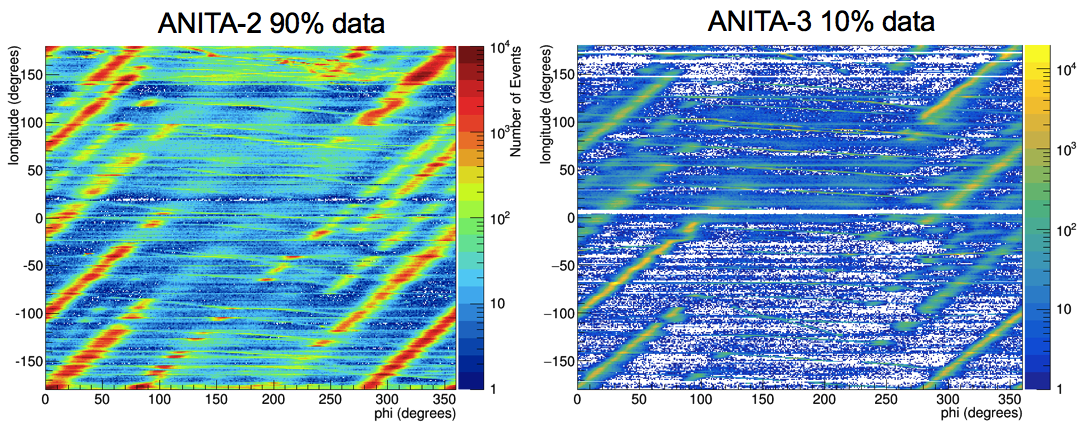
\includegraphics[width=1.0\textwidth]{figures/same_stripes.png}
\caption{Satellite stripe plots for the ANITA-2 and ANITA-3 flights.}
\label{sat_stripe}
\end{figure}

\section{Code for satellite stripe plot}

Example code used to make the satellite stripe plot for the \gls{anita}-3 and -2 flights are shown below. The \gls{anita}-3 code is a macro and runs independent of other \gls{anita} software. It needs to be run on Oakley as the \gls{anita}-3 data is located there. The \gls{anita}-2 code is meant to be compiled and run inside the \path{anita2code} directory of the binned analysis software which is located at:
\href{https://github.com/osu-particle-astrophysics/BinnedAnalysis}{https://github.com/osu-particle-astrophysics/BinnedAnalysis}. 

The code to make the \gls{anita}-3 satellite stripe plot is a macro called \path{plotLonPhi}. A macro is a piece of code in ROOT meant to serve only one function. Inside the macro, that function is written and the name of the macro is the same as the name of the function. 
In this particular macro, first I declare a TChain object. A TChain object is a collection of files containing TTrees. This is useful in \gls{anita} as you can add together the TTrees associated with data files of multiple runs into one object. To make the satellite stripe plot for \gls{anita}-3, we use the output files from runInterferometry.cxx of the \gls{anita}-3 binned analysis. These are saved as multiple ROOT files, one file per run. 

I used the 10\% data to make the \gls{anita}-3 plot. To use the 90\% data, change \path{sample_10} in the directory name to \path{sample_90}. Note that Draw, a member function of both TTree and TChain, is used. This allows one to make the plot without including the classes that data objects inherit from. The function Draw accesses what is inside the TTree directly without requiring a definition of the data type inside the tree. The plot can also be made in the traditional way of filling a histogram with entries from a TChain inside a for loop. 

The idea behind making the satellite stripe plot for \gls{anita}-2 is the same, however, the \gls{anita}-2 analysis software is unique. 
\gls{anita}-2 data is on Kingbee and that is where \path{anita2code} have been run and tested. The code to make the satellite stripe plot for \gls{anita}-2 is part of \path{oindreeskymap.cc} in \path{anita2code}. Note the \path{.h} files that must be included to run this code, especially \path{analysis_info_4pol.h}, which is a struct holding the necessary data variables. 


\par
\begin{verbbox}
/////////////////////FOR ANITA-3///////////////////////
void plotLonPhi();

void plotLonPhi()

{
  //Declare a TChain object (collection of files containing TTrees)
  TChain tchain("resultTree");
  
  //Add files containing data processed by interferometry
  tchain.Add("/fs/scratch/PAS0174/anita
  /2015_05_19/sample_10/geomFilter/analyzerResults_*.root");

  //Declare a TH2D object 
  //First argument is the name of the histogram
  //which is same as the variable name here 
  TH2D hlonPhi00("hlonPhi00","ANITA-3 10% Data LPol;
  phi (degrees);longitude (degrees)",360,0,360,360,-180,180);
  
  //Declare a TCanvas object 
  //which is needed to make a plot in ROOT
  TCanvas cL("cL","cL",900,800);
  
  //Use the Draw function to plot the histogram
  //TTree and TChain have this useful function Draw 
  //Draws and puts the histogram in the TH2D object you specified
  tchain.Draw("longitude:(fmod((peak[0][0].phi - heading + 360),360)) 
  >> hlonPhi00", "circPol == 1", "colz");
  //Set the color axis to log scale
  cL.SetLogz();
  //Save plot as a .png (or other chosen format)
  cL.SaveAs("LonPhiPeak00CPol1.png");
  //Save plot as .root as well for quick changes as needed
  cL.SaveAs("LonPhiPeak00CPol1.root");
  
}
\end{verbbox}
\fbox{\theverbbox}\par

\par
\begin{verbbox}
/////////////////////FOR ANITA-2///////////////////////
#include "analysis_info_4pol.h" //struct holding data variables 
using namespace std;
class MyCorrelator;
int main()
{
  char filename90[10000];
  char filename10[10000];
  sprintf(filename90,"/data/anita/btdailey/final_filter/
  90sample/geom_4pol_partial_0301/output*000.root");
  sprintf(filename10,"/data/anita/btdailey/final_filter/
  10sample/geom_4pol_partial_0301/output*.root");
  TChain tchain("analysis_info_4pol");
  tchain.Add(filename90);
  tchain.Add(filename10);
  
  //Create a pointer to instantiate struct 
  analysis_info_4pol *pol4_Ptr = NULL;
  tchain.SetBranchAddress("pol4_Ptr",&pol4_Ptr);
  
  //Note: R & L are switched in ANITA-2
  TH2D LonPhiR("LonPhiR","ANITA-2 100% Data After Quality Cuts;
  phi (degrees); longitude (degrees)", 360,0,360,360,-180,180);
  
  TCanvas cRmap("cRmap","cRmap",1000,800);
  tchain.Draw("pol4_Ptr->anitaLon:
  (fmod((pol4_Ptr->phiMap[3]-pol4_Ptr->heading+360),360)) 
  >> LonPhiR","","colz"); //R & L are switched in ANITA-2
  
  cRmap.SetLogz();
  cRmap.SaveAs("LonPhiR100pc.png");
  cRmap.SaveAs("LonPhiR100pc.root");
}
\end{verbbox}
\fbox{\theverbbox}